\section{Fixation du rail magnétique}\label{FixRailMag}
Un problème est survenu lors de la fixation du rail magnétique du moteur sur un des profilés. La partie inférieure du rail est trop courte
pour correctement s'appuyer sur le profilé et le rail rentre dans la rainure lorsqu'il est vissé. La situation est visible sur l'image ci-dessous.

\begin{figure}[H]
    \centering
    \includegraphics[width = 0.4\textwidth]{assets/figures/FixationRailMagProb.png}
    \caption{Illustration du problème de fixation du rail magnétique}
    \label{fig:FixRailMagProb}
\end{figure}

La solution apportée à ce problème est l'utilisation de plaques de fixations placées entre le rail et le profilé. Ceci va permettre de répartir
la charge de chaque côté de la rainure et d'empêcher le rail de pencher en rentrant dans la rainure. Les représentations des deux plaques créées
sont illustrées ci-dessous.

\begin{figure}[H]
    \centering
    \includegraphics[width = 0.7\textwidth]{assets/figures/PlaqueFixation1.svg}
    \caption{Illustration de la première plaque de fixation pour le rail magnétique}
    \label{fig:PlaqueFix1}
\end{figure}

\begin{figure}[H]
    \centering
    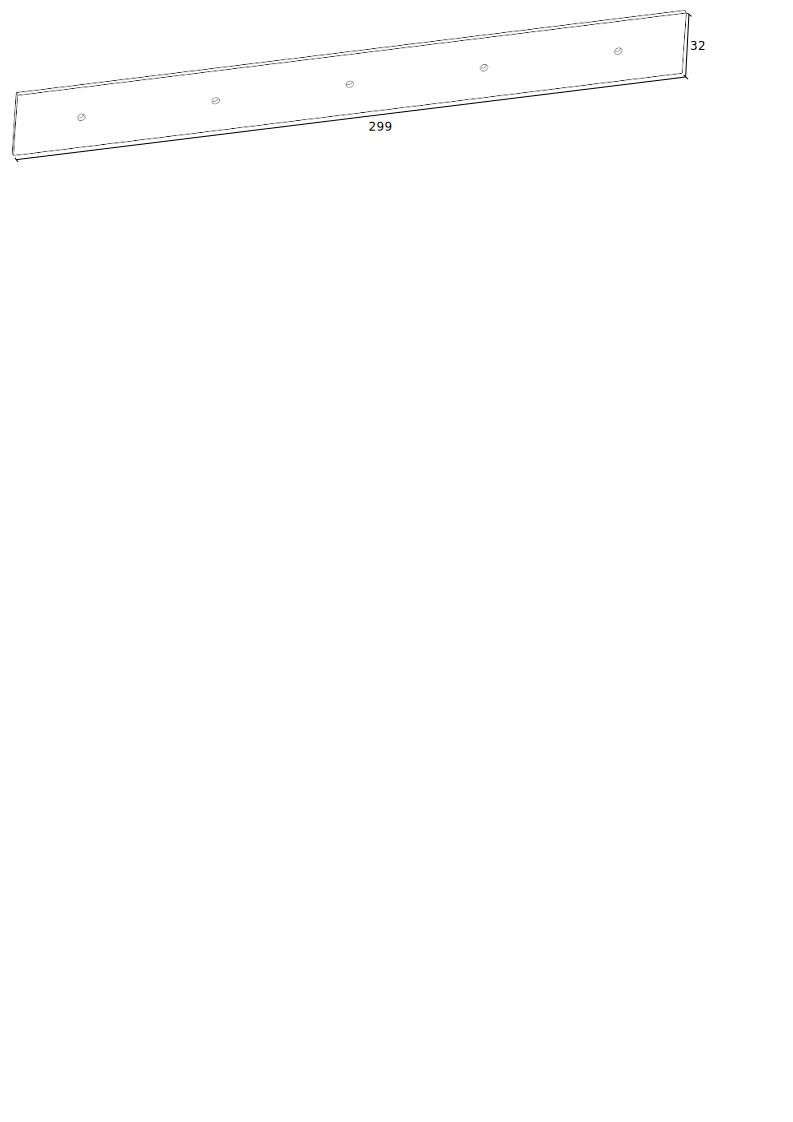
\includegraphics[width = 0.9\textwidth]{assets/figures/PlaqueFixation2.svg}
    \caption{Illustration de la seconde plaque de fixation pour le rail magnétique}
    \label{fig:PlaqueFix2}
\end{figure}

La figure suivante illustre la solution appliquée et comment elle résout le problème.

\begin{figure}[H]
    \centering
    \includegraphics[width = 0.4\textwidth]{assets/figures/FixationRailMagSol.png}
    \caption{Illustration de la solution de fixation du rail magnétique}
    \label{fig:FixRailMagSol}
\end{figure}

Cependant, cette modification éloigne le rail magnétique de 2~mm du chariot. Il faut donc modifier la pièce de liaison au moteur pour la ralonger
de 2~mm aussi. Le support de la tête de lecture de la règle linéaire est aussi décalée afin de maintenir la position de la tête de lecture.